\documentclass[../main.tex]{subfiles}

\begin{document}

\textbf{Trường điều kiện ngẫu nhiên - Conditional Random Field (CRF) }

CRF là mô hình giúp xử lý bài toán về chuỗi tương đối giống với mô hình HMM. Mô hình CRF có tất cả ưu điểm của HMM và tránh được vấn đề thiên vị cho nhãn của mô hình cực đại hóa entropy Markov (MEMM) (\cite{mccallum2000maximum}). 

Mục đích của mô hình là học hàm ánh xạ $x_{s} \rightarrow y_{s}$. Tuy nhiên mỗi đầu ra $y_{s}$ không độc lập với nhau. Mô hình CRF có khả năng dự đoán vector đầu ra $y = y_{0}, y_{1}, ..., y_{t}$ thông qua tính toán xác suất có điều kiện của các biến ngẫu nhiên đưa ra trong vector quan sát là $x = x_{0}, x_{1}, ..., x_{t}$ (\cite{sutton2012introduction})
Mô hình CRF kết hợp phân loại phân biệt và mô hình xóa bằng đồ thị. Nhờ thế mà có thể mô hình hóa các đặc trưng một cách gọn gàng vầ sử dụng lượng lớn các thông tin đầu vào cho việc dự đoán. (\cite{sutton2012introduction})

Mô hình CRF cũng được áp dụng cho nhiều lĩnh vực. Ví dụ như việc xử lý ngôn ngữ hay tiếng nói như bài toán gán nhãn từ (\cite{ghosh2016part}), NER (\cite{seker2017extending}), trích xuất thông tin (\cite{ebersbach2016wrappers} hay giải quyết mập mờ về ngữ pháp (\cite{radziszewski2013tiered}). Trong Tin sinh học, các ứng dụng CRF có thể kể đến là tìm ra liên kết protein (\cite{morales2018protein}), khám phá và dự đoán cấu trúc RNA \cite{johansen2017deep}. 

Để mô tả mô hình CRF bằng đồ thị, gọi $G = (V,  E)$ là một đồ thị. $V$ biểu diễn tập đỉnh, $E$ biểu diễn tập cạnh nối trực tiếp giữa 2 đỉnh. Mỗi đỉnh $\nu$ được gán một biến $Y_{v}$, thế nên $Y = (Y_{v})\nu \in V$, với mọi $Y_{v}$ tuân theo tính chất của Markov. Nhờ vậy mà cả mô hình đồ thị có thể mô tả bằng biểu thức sau: (\cite{lafferty2001conditional})

\begin{equation}
P(Y_{v}|X, Y_{w}, w \neq \nu) = P(Y_{v}|X, Y_{w}, w \sim v) \nonumber
\end{equation}

Trong đó, $ w \sim v$ có nghĩa rằng $w$ và $v$ kết nối với nhau trong $G$. 

Điều cần chú ý trong CRF là việc mô phỏng CRF thì lại dùng fđồ thị vô hướng. Vì thế, trong xử lý ngôn ngữ tự nhiên, các nhà nghiên cứu đã sử dụng chuỗi tuyến tính CRF  \cite{yu2019named}. 

\begin{figure}[h]
\centering
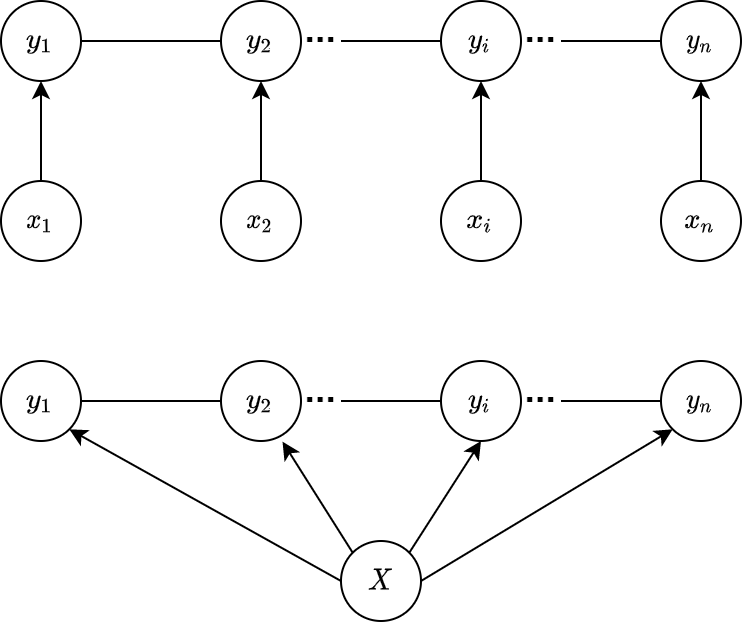
\includegraphics[scale=0.4]{02-LN-CRF}
\caption{Cấu trúc của mô hình chuỗi tuyến tính CRF}
\end{figure}

Với bài toán nhận diện tên thực thể cũng thường sử dụng chuỗi tuyến tính CRF. Cấu trúc của chuỗi được nêu ra ở trên. Các đỉnh được gộp vào cấu trúc chuỗi tuyến tính, và chuỗi các đỉnh này tạo ra tương ứng với chuỗi $Y$. Khi cho một biến ngẫu nhiên $X = x_{1}, x_{2}, ..., x_{n}$ cùng $Y = y_{1}, y_{2}, ..., y_{n}$ với cấu trúc chuỗi tuyến tính thì phân phối xác suất có điều kiện của biến ngẫu nhiên $Y$ là $P(Y|X)$ cũng tuân theo tính chất Markov. 

\begin{equation}
P(y_{i}|x, y_{1}, y_{2}, ..., y_{n}) = P(y_{i}|x, y_{i-1}, y_{i+1}) \nonumber
\end{equation}

Vì thế, với chuỗi quan sát $X$, ta có thể sử dụng phân phối $P(Y|X)$ của biến ngẫu nhiên Y để dự đoán chuỗi Y \cite{wallach2004conditional}
\end{document}